% Glueball A0 landscape poster, built on the CASCADE Beamer theme.
% Build:  latexmk -pdf glueball-poster.tex
\documentclass[final]{beamer}
\usepackage[size=a0,orientation=portrait,scale=0.85]{beamerposter}
\usetheme{Cascade}
\setbeamerfont{title}{size=\huge,series=\cascadeheadfont}
\setbeamerfont{author}{size=\large,series=\bfseries}
\newlength{\cascadegap}\setlength{\cascadegap}{0.6cm}
\usepackage{adjustbox}
\usepackage{booktabs,array,listings,multirow,colortbl}
\usetikzlibrary{arrows.meta,positioning,calc,fit}

\definecolor{okgreen}{HTML}{2A7A62}
\definecolor{bad}{HTML}{A8483C}
\newcommand{\good}[1]{{\color{okgreen}#1}}
\newcommand{\poor}[1]{{\color{bad}#1}}
\newcommand{\best}[1]{\cellcolor{cascadered!22}\textbf{#1}}

\definecolor{codeblue}{HTML}{2F5E9E}
\definecolor{codegreen}{HTML}{2A7A62}
\definecolor{codegrey}{HTML}{8A8F9C}
\lstdefinelanguage{z3out}{morekeywords={DATA,RACE,STORE,LOAD,PIPELINE,COLLISION},sensitive=true}
\lstset{basicstyle=\ttfamily\scriptsize,columns=fullflexible,keepspaces=true,
  language=Python,showstringspaces=false,breaklines=true,
  keywordstyle=\color{cascadered}\bfseries,
  commentstyle=\color{codegrey}\itshape,
  stringstyle=\color{codegreen},
  numberstyle=\color{codegrey},
  emph={GluonVerificationContext,map_async_copy_global_to_shared,map_async_commit_group,map_async_wait_group,map_load,program_order,check_async_race_freedom,wait_group,perform_add},
  emphstyle=\color{codeblue}\bfseries,
  frame=single,rulecolor=\color{cascadelightgrey!60},backgroundcolor=\color{white},
  framesep=0.7em,xleftmargin=0.7em,xrightmargin=0.7em,aboveskip=0.15em,belowskip=0.15em}

% ---- unified table style: red header, alternating peach rows, thin red rule
\newcommand{\hd}[1]{\textcolor{white}{\bfseries #1}}
\newcommand{\tablestyle}[1]{\renewcommand{\arraystretch}{1.3}\setlength{\tabcolsep}{9pt}%
  \rowcolors{#1}{white}{cascadepeach!45}\arrayrulecolor{white}}

\tikzset{
  nd/.style={draw=cascadelightgrey,rounded corners=3pt,thick,align=center,
    minimum height=3.2cm,inner xsep=0.5cm,fill=white,font=\large},
  tr/.style={nd,fill=cascadepeach},
  ok/.style={nd,draw=okgreen,fill=okgreen!12},
  bd/.style={nd,draw=cascadered,fill=cascadered!10,dashed},
  ar/.style={-{Stealth[length=3mm]},thick,draw=cascadegrey},
  rj/.style={-{Stealth[length=3mm]},thick,draw=cascadered,dashed},
}

\title{Glueball: Agentic Generation and Verification of Hardware-Optimized Gluon Kernels}
\author{Yash Shah, Mantas Baksys,\\Sean B.\ Holden, Timothy M.\ Jones}
\institute{ICLR 2027 submission}
\event{Glueball \textperiodcentered{} ICLR 2027 submission}
\contact{Yash Shah, Mantas Baksys, Sean B.\ Holden, Timothy M.\ Jones}
\supporters{}
\qrurl{https://www.cl.cam.ac.uk/research/cascade/}
\takeaway{Theorem-proving tools help LLM agents find more kernel bugs, with fewer false positives and fewer tokens.}

\begin{document}
\begin{frame}[t,fragile]
\begin{columns}[t,totalwidth=\linewidth]
\begin{column}{0.58\linewidth}
  \begin{block}{Motivation and contributions}
    Tests cover little of the execution space, so agents can \alert{overfit to tested inputs} and miss races and barrier bugs in asynchronous Hopper/Blackwell kernels.
    \begin{itemize}
      \item \textbf{Glueball} is the first system to equip LLM agents with \textbf{theorem-proving tools} during GPU kernel generation.
      \item It targets \textbf{Gluon}, Triton's tile-level DSL with explicit layouts and warp roles, whose structure suits formal reasoning.
      \item Agents get profilers, debuggers and compilers, Z3 via our Gluon-to-Z3 library, and are judged on whole models.
    \end{itemize}
  \end{block}
\end{column}
\begin{column}{0.38\linewidth}
  \begin{alertblock}{IN ONE SENTENCE}
    Theorem-proving tools help LLM agents find more kernel bugs, with fewer false positives and fewer tokens.
  \end{alertblock}
\end{column}
\end{columns}
\vskip\cascadegap
\begin{columns}[t,totalwidth=\linewidth]
\begin{column}{0.485\linewidth}
  \begin{block}{System: optimize, verify, benchmark}
    \centering
    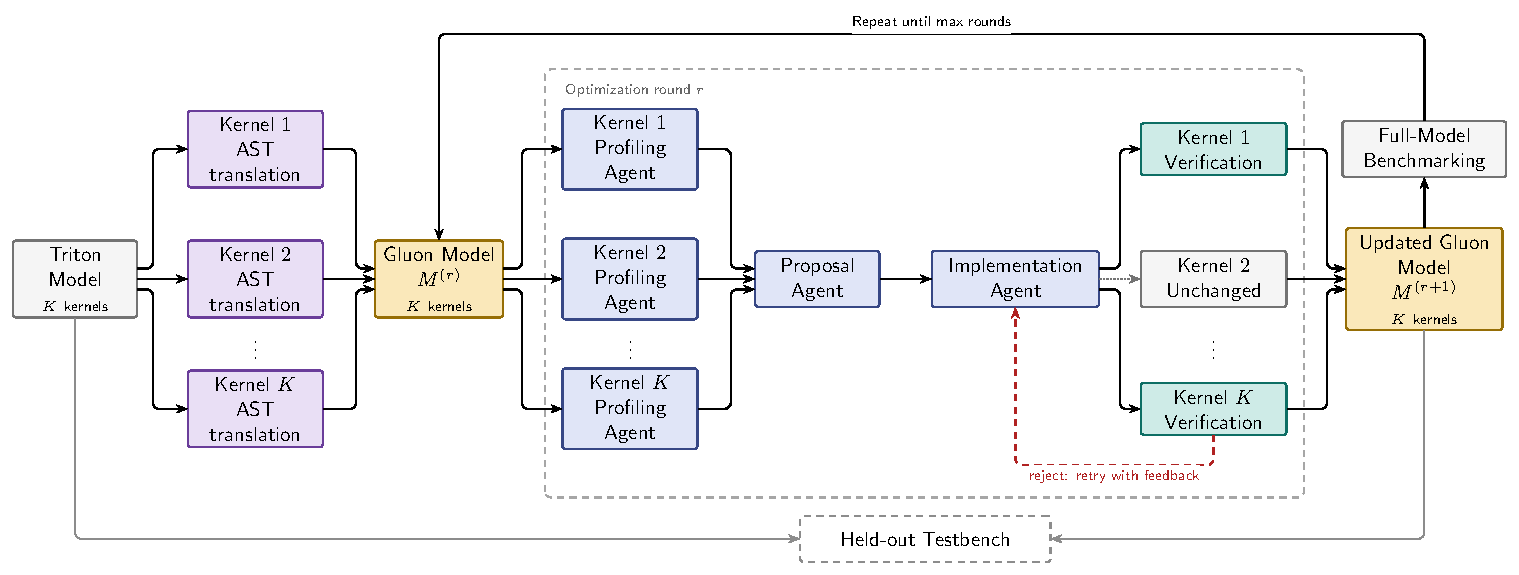
\includegraphics[width=\linewidth]{diagrams/model_pipeline.pdf}
  \end{block}
\end{column}
\begin{column}{0.485\linewidth}
  \begin{block}{Correctness pipeline}
    \centering
    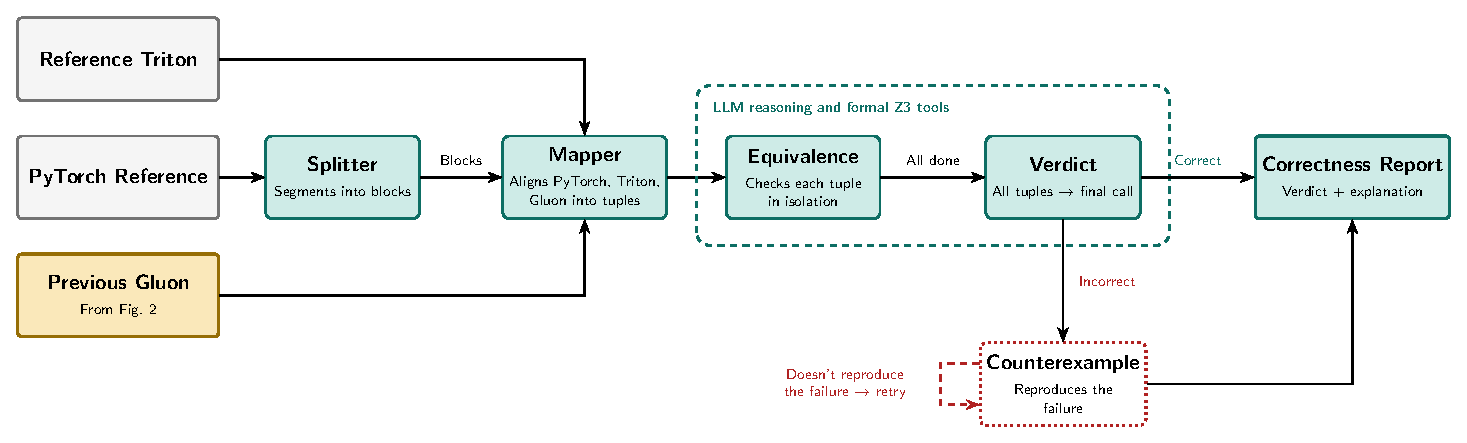
\includegraphics[width=\linewidth]{diagrams/correctness_detail.pdf}
  \end{block}
\end{column}
\end{columns}
\vskip\cascadegap
\begin{columns}[t,totalwidth=\linewidth]
\begin{column}{0.485\linewidth}
  \begin{block}{Whole-model speedups}
    \centering\small
    \adjustbox{width=0.6\linewidth,center}{\tablestyle{2}\begin{tabular}{llccccc}
      \rowcolor{cascadered}\rule[-2.2ex]{0pt}{6.4ex}\hd{Workload} & \hd{Type} & \hd{\shortstack[c]{Astra\\+CODEX}} & \hd{\shortstack[c]{DeepSeek\\V4 Pro}} & \hd{\shortstack[c]{DeepSeek\\V4 Flash}} & \hd{\shortstack[c]{Meta Muse\\Spark 1.3}} & \hd{\shortstack[c]{GPT\\5.6 Sol}}\\
      GPT-OSS & Model & \best{\good{1.13$\times$}} & \good{1.067$\times$} & \poor{0.891$\times$} & \poor{0.914$\times$} & \poor{0.921$\times$}\\
      Qwen-3.5 MoE & Model & \poor{0.99$\times$} & \good{1.066$\times$} & \best{\good{1.075$\times$}} & \poor{0.997$\times$} & \poor{0.851$\times$}\\
      Mamba-2 & Model & \best{\good{1.00$\times$}} & \poor{0.990$\times$} & \poor{0.958$\times$} & \poor{0.957$\times$} & \poor{0.958$\times$}\\
      Cross-Entropy & Kernel & \good{1.02$\times$} & \good{1.550$\times$} & \poor{0.980$\times$} & \poor{0.820$\times$} & \best{\good{1.669$\times$}}\\
      Llama-4 RoPE & Kernel & \best{\good{1.10$\times$}} & \good{1.073$\times$} & \good{1.069$\times$} & \good{1.011$\times$} & \good{1.047$\times$}\\
      Neighborhood Att. & Kernel & \good{4.69$\times$} & \good{23.077$\times$} & \best{\good{24.851$\times$}} & \good{24.529$\times$} & \good{24.521$\times$}\\
      \arrayrulecolor{cascadered}\bottomrule
    \end{tabular}}
    \par\vskip0.4em{\footnotesize\color{cascadegrey}Median best-round speedup (GB10, 6 rounds); shaded = best.}
  
  \end{block}
\end{column}
\begin{column}{0.485\linewidth}
  \begin{block}{Verification finds more bugs}
    \centering\small
    \adjustbox{width=0.6\linewidth,center}{\tablestyle{3}\begin{tabular}{lcccccccc}
      \rowcolor{cascadered} & \multicolumn{4}{c}{\hd{Generic suite}} & \multicolumn{4}{c}{\hd{Sync suite}}\\
      \cmidrule(lr){2-5}\cmidrule(lr){6-9}
      \rowcolor{cascadered}\hd{Model} & \hd{Bugs$\uparrow$} & \hd{$\Delta$} & \hd{FP$\downarrow$} & \hd{$\Delta$} & \hd{Bugs$\uparrow$} & \hd{$\Delta$} & \hd{FP$\downarrow$} & \hd{$\Delta$}\\
      DeepSeek V4 Pro & 21 & \good{+3} & 0 & 0 & 10 & 0 & 7 & \good{$-$5}\\
      DeepSeek V4 Flash & 22 & \good{+2} & 0 & 0 & 10 & 0 & 1 & \good{$-$1}\\
      Meta Muse Spark 1.3 & 22 & \good{+2} & 0 & 0 & 9 & 0 & 3 & \good{$-$3}\\
      GPT 5.6 Sol & 21 & \good{+2} & 0 & 0 & 9 & \good{+1} & 1 & \good{$-$1}\\
      \arrayrulecolor{cascadered}\bottomrule
    \end{tabular}}
  
  \end{block}
\end{column}
\end{columns}
\vskip\cascadegap
  \begin{block}{Ablation: what do the tools buy?}
    \centering\small
\begin{columns}[t,totalwidth=\linewidth]
\begin{column}{0.6\linewidth}
\adjustbox{width=0.62\linewidth,center}{\tablestyle{3}\begin{tabular}{lccccc}
      \rowcolor{cascadered} & \multicolumn{2}{c}{\hd{Bug detection}} & \multicolumn{3}{c}{\hd{Bug-free code}}\\
      \cmidrule(lr){2-3}\cmidrule(lr){4-6}
      \rowcolor{cascadered}\hd{Test arm} & \hd{Found/30} & \hd{Tokens} & \hd{FP/21} & \hd{Tokens} & \hd{Tool calls}\\
      Both tools & \good{28} & \good{0.93 M} & \good{0} & 3.63 M & 47.6\\
      Z3 library only & \good{28} & 1.21 M & \good{0} & \good{3.52 M} & \good{43.6}\\
      Symbolic exec.\ only & 27 & 1.40 M & \good{0} & 4.29 M & 50.9\\
      Neither (raw model) & 27 & 1.52 M & \poor{7} & 4.44 M & 71.2\\
      \arrayrulecolor{cascadered}\bottomrule
    \end{tabular}}
\end{column}
\begin{column}{0.37\linewidth}
\adjustbox{width=0.72\linewidth,center}{\tablestyle{2}\begin{tabular}{lcccc}
      \rowcolor{cascadered}\hd{Tokens per defect} & \hd{Both} & \hd{Z3 only} & \hd{Symexec only} & \hd{Neither}\\
      \texttt{cpasync\_barrier} & \good{0.42 M} & 0.62 M & 1.47 M & \poor{1.75 M}\\
      \texttt{arrive\_before\_fence} & 1.24 M & \good{0.90 M} & 3.19 M & \poor{3.69 M}\\
      \texttt{missing\_fence} & \good{1.77 M} & 2.05 M & 2.68 M & \poor{3.33 M}\\
      \arrayrulecolor{cascadered}\bottomrule
    \end{tabular}}
    \par\vskip0.4em{\footnotesize\color{cascadegrey}DeepSeek V4 Pro (high), tools tested in isolation.}
  
\end{column}
\end{columns}
  \end{block}
\vskip\cascadegap
  \begin{block}{Case study: a pipelining bug}
\begin{columns}[t,totalwidth=\linewidth]
\begin{column}{0.235\linewidth}
    \textbf{\color{cascadedarkred}(a) The bug}
\begin{lstlisting}
# Correct
cp.wait_group(num_buffers - 1)
# Bug
cp.wait_group(num_buffers)
perform_add(
    a_smem[i % num_buffers],
    b_smem[i % num_buffers])
\end{lstlisting}
\end{column}
\begin{column}{0.235\linewidth}
    \textbf{\color{cascadedarkred}(b) Symbolic model}
\begin{lstlisting}
ctx.map_async_copy_global_to_shared(
    0, src_addr=0x1000,
    dst_addr=0x100, size=4,
    label='copy0')
...
wait = ctx.map_async_wait_group(
    0, num_outstanding=wait_arg,
    label=f'wait({wait_arg})')
load = ctx.map_load(
    0, 0x100, Space.SHARED,
    size=4, label='read buffer0')
ctx.program_order(wait.id, load.id)
safe, model = (
    ctx.check_async_race_freedom())
\end{lstlisting}
\end{column}
\begin{column}{0.235\linewidth}
    \textbf{\color{cascadedarkred}(c) Z3 verdict}
\begin{lstlisting}[language=z3out]
wait_group(2):
DATA RACE detected:
  copy0.smem_write
    STORE SHARED@0x100
    proxy=ASYNC_COPY
  <-race->
  read buffer0
    LOAD SHARED@0x100
    proxy=GENERIC
\end{lstlisting}
\end{column}
\begin{column}{0.235\linewidth}
    \textbf{\color{cascadedarkred}(d) Pipeline witness}
\begin{lstlisting}[language=z3out]
check_pipeline_stage_isolation(
    num_stages=2, max_inflight=2)
PIPELINE COLLISION:
producer and consumer share a slot
witness: [iter_p = 2, lag = 2]
\end{lstlisting}
\end{column}
\end{columns}
  \end{block}
\vskip\cascadegap
\begin{columns}[t,totalwidth=\linewidth]
\begin{column}{0.485\linewidth}
  \begin{block}{Symbolic execution: TTIR to Z3}
    Each MLIR op becomes a Z3 term; ops the model cannot capture become \alert{fresh opaque symbols} that split the kernel into \alert{symbolic regions}. Softmax example:
    \vskip0.6em
    \centering\small
    \adjustbox{width=0.62\linewidth,center}{\tablestyle{2}\begin{tabular}{lll}
      \rowcolor{cascadered}\hd{TTIR op} & \hd{Z3 term} & \hd{Kind}\\
      \texttt{tt.load} & \texttt{load\_row} & fresh symbol\\
      \texttt{tt.reduce (max)} & \texttt{maxnumf\_row\_minus\_max} & fresh symbol\\
      \texttt{arith.subf} & \texttt{load\_row - maxnumf\_\dots} & \texttt{fpSub}\\
      \texttt{math.exp} & \texttt{exp(load\_row - \dots)} & uninterpreted fn\\
      \texttt{tt.reduce (sum)} & \texttt{addf\_denominator} & fresh symbol\\
      \texttt{arith.divf} & \texttt{exp(\dots) / addf\_denominator} & \texttt{fpDiv}\\
      \arrayrulecolor{cascadered}\bottomrule
    \end{tabular}}
  \end{block}
\end{column}
\begin{column}{0.485\linewidth}
  \begin{block}{The Gluon-to-Z3 library}
    Hardware actions become \alert{events} ordered by \emph{happens-before}. Each \emph{theorem} asks Z3 to satisfy the \alert{negation} of a property: \textbf{UNSAT} proves it, \textbf{SAT} gives a counterexample.
    \vskip0.6em
    \centering\small
    \adjustbox{width=0.66\linewidth,center}{\tablestyle{2}\begin{tabular}{ll}
      \multicolumn{2}{l}{\cellcolor{cascadered}\hd{Axioms: hardware ordering rules}}\\
      Sequential consistency & events form an acyclic timeline\\
      CTA barrier & \texttt{gl.barrier()}: before $\Rightarrow$ after, all threads\\
      Async-proxy fence & orders generic writes before TMA / MMA reads\\
      Mbarrier sync & arrival and byte accounting; short $\Rightarrow$ deadlock\\
      Manual ordering & assert or deny a happens-before edge\\
      \multicolumn{2}{l}{\cellcolor{cascadered}\hd{Theorems: safety properties}}\\
      Async race freedom & no unordered access pair with a write\\
      Bank-conflict freedom & same-warp threads hit distinct banks\\
      Global coalescing & warp accesses fit one aligned cache line\\
      \arrayrulecolor{cascadered}\bottomrule
    \end{tabular}}
  \end{block}
\end{column}
\end{columns}
\vskip\cascadegap
  \begin{block}{Future directions}
\begin{columns}[t,totalwidth=\linewidth]
\begin{column}{0.31\linewidth}
\begin{itemize}\item \textbf{Multi-GPU and heterogeneous targets.} Distributed kernels (ParallelKernelBench) and other accelerators, with proof obligations for collective ordering and distributed races.\end{itemize}
\end{column}
\begin{column}{0.31\linewidth}
\begin{itemize}\item \textbf{Constraint- and statistics-guided search.} Prune pipelining schedule families before codegen; use past feedback to cut costly LLM iterations.\end{itemize}
\end{column}
\begin{column}{0.31\linewidth}
\begin{itemize}\item \textbf{Verification across the compilation stack.} Further formal tools, such as a formal PTX model, to verify at several levels (Gluon, TTGIR, PTX).\end{itemize}
\end{column}
\end{columns}
  \end{block}
\end{frame}
\end{document}
